\chapter{Josephus problem}
\section{Indledning}
Et klassisk problem som angiveligt stammer fra det første århundrede. Under den jødisk-romerske krig var 41 jødiske oprørere fanget i en hule. Situationen var kritisk og gruppen besluttede at begå kollektivt selvmord ved at stille sig i en cirkel og herefter gå frem og dræbe hver tredie indtil alle var dræbt undtagen en. Han skulle så begå selvmord. Josephus var ikke enig i denne selvmordspaln og regnede hurtigt ud hvor han skulle placere sig i cirklen for at overleve som sidste mand. Men hvordan regnede han det ud?
Istedet for at stille folk i en cirkel, sætter vi dem nu på række. Vi tager et eksempel med 10 personer, hvor hver tredie bliver dræbt. Når en person er sprunget over, altså har undgået at blive dræbt stiller han sig forrest i køen og venter at bøddelen kommer igen.
\section{Basismodel}
For bedre at kunne regne på problemet indfører vi følgende parametre
\begin{alignat*}{2}
&q=3 \quad &&\text{Frekvensen med hvilken bøddelen slår til.}\\
&n=10 \quad &&\text{Antal personer}\\
&k \quad &&\text{Antal der er slået ihjel}\\
&n-k \quad &&\text{Antal personer der er tilbage}
\end{alignat*}
Bøddelen går systematisk frem og henretter hver tredie (\(q=3\)). Hvis man således kommer til at stå på et felt hvor 3 går op i nummeret er man dødsdømt. Når bøddelen har passeret nr.\(1\) går nr. \(1\) forrest i rækken og får et nyt nummer - i dette tilfælde nr.\(11\). Første gang bøddelen passerer nr.\(1\) er der ikke elimineret nogle (\(k=0\)) og person nr.\(1\) må gå \(10\) pladser frem til nr.\(11\) fordi der er \(10\) personer tilbage (\(n-k=10\)). Der gælder derfor generelt:
\begin{equation}
N_{ny}=N_{gammel}+(n-k)\label{Nny}
\end{equation}
For eksempel ses det, at person nummer \(7\) i næste omgang får nummer \(15\), da der er elimineret \(2\) personer (\(k=2\)) og \(N_{ny}=7+(10-2)=7+8=15\). (Det er synd for ham, da 3 går op i \(15\) og han dermed henrettes næste gang.)\\
Bøddelen går videre og til sidst eliminerer han personen med nr.\(27\) og der er kun en mand tilbage. Der er elimineret 9 personer og det tager 9 henrettelser at komme til person nr.\(27\) med en henrettelsesfrekvens på 3 (\(q=3\)). Hvis vi fortsætter må sidste mand hver gang gå et felt frem indtil han når felt \(30\), vor han henrettes. Dette svarer til 10 henrettelser.
\section{Beregne vinderen}
Hvis vi nu kan gå baglæns fra feltet \(30=nq\) og finde ud af hvilket nr. denne person startede på, har vi nummeret på vinderen. Vi kan udtrykke alle de personer, der bliver sprunget over på formen \(3k+a\), hvor \(a=1\) eller \(a=2\) - \(a\) vil altid være et helt tal hvorom der gælder at \(0<a<q\). En person med 
\[N_{gammel}=3k+a\] 
bliver altså sprunget over og får et nyt nummer. Ved omskrivning fås:
\begin{equation}
k=\frac{N_{gammel}-a}{3}=\frac{N_{gammel}-a}{q}\label{klign}
\end{equation}
, hvor
\[0 < a < q\]
Indsætter vi nu \ref{klign} i \ref{Nny} fås:

\begin{alignat}{2}
&&&N_{ny}=N_{gammel}-n-\frac{N_{gammel}}{q}+\frac{a}{q}\\
\ArrowBetweenLines
&&&N_{gammel}(1-\frac{1}{q})=N_{ny}-n-\frac{a}{q}\\
\ArrowBetweenLines
&&&N_{gammel}(\frac{q-1}{q})=N_{ny}-n-\frac{a}{q}\\
\ArrowBetweenLines
&&&N_{gammel}=\frac{q}{q-1}(N_{ny}-n)-\frac{a}{q-1}\label{gammel}
\end{alignat}

Da \(0 < a < q\) er den største værdi a kan antage \(a_{max}=q-1\). Herved ses det, at:
\[0 < \frac{a}{q-1} \leq 1\], hvor lighedstegnet gælder når \(a=q-1\).

Vi kan afprøve \ref{gammel} og ønsker at finde startfeltet for ham som står på felt \(22\). Vi har \(q=3, N_{ny}=22, n=10\) og vi får:
\[N_{gammel}=\frac{3}{2}(22-10)-\frac{a}{2}=18-\frac{a}{2}\]
\(N_{gammel}\) må være et helt tal, så \(a=2\) og \(N_{gammel}=18-1=17\). Da \(17>n=10\) er dette ikke startnummeret, så vi går videre:

\[N_{ny}=17: \quad N_{gammel}=\frac{3}{2}(17-10)-\frac{a}{2}=\frac{21}{2}-\frac{a}{2}\]

Da a=1 \(\lor\) a=2 og \(N_{gammel}\) er et helt tal må \(a=1\) og vi får \(N_{gammel}=\frac{21}{2}-\frac{1}{2}=10\). Dette var altså startfeltet for ham der stod på felt \(22\). Vi ønsker nu at finde startfeltet for overleveren der ender på felt \(30\). Den næstesidste overlever døde på felt \(27\), så overleveren må have stået på felt \(26\) eller generelt på felt \(nq-q-1\). Dette sparer os for et par udregninger:

\begin{align*}
&N_{ny}=26 \quad \Rightarrow N_{gammel}=\frac{3}{2}(26-10)-\frac{a}{2}=24-\frac{a}{2}=23\\
&N_{ny}=23 \quad \Rightarrow N_{gammel}=\frac{3}{2}(23-10)-\frac{a}{2}=\frac{39}{2}-\frac{1}{2}=19\\
&N_{ny}=19 \quad \Rightarrow N_{gammel}=\frac{3}{2}(19-10)-\frac{a}{2}=\frac{27}{2}-\frac{1}{2}=13\\
&N_{ny}=13 \quad \Rightarrow N_{gammel}=\frac{3}{2}(13-10)-\frac{a}{2}=\frac{9}{2}-\frac{1}{2}6=4
\end{align*}
Det var altså nummer \(4\) i rækken der overlevede i tilfældet \(q=3, n=10\).
Vi regnede baglæns fra \ref{gammel} ved at indsætte aktuel \(N_{ny}\). Lad os prøve at indsætte \(N_{ny}=nq-1\), hvor \(N_{ny}\) udtrykkes i form af afstanden \(d\) fra sidste elimineringsfelt. I eksemplet er \(nq=10 \cdot 3 =30\) og \(N_{ny}=26=30-d=30-4\). Vi indsætter \(N_{ny}=nq-d\) i \ref{gammel} og får:
\begin{align}
N_{gammel}&=\frac{q}{q-1}(nq-d-n)-\frac{a}{q-1}\\
&=\frac{q}{q-1}(n(q-1)-d)-\frac{a}{q-1}\\
&=nq-\frac{qd}{q-1}-\frac{a}{q-1}
\end{align}
Eksemplet med overleveren vil nu se sådan ud:

\[N_{ny}=26, d_{ny}=4\]
\[ N_{gammel}=30-\frac{3}{2} \cdot 4 -\frac{a}{2}=30-6-1=30-7=23\]
\[N_{ny}=23, d_{ny}=7\]
\[ N_{gammel}=30-\frac{3}{2} \cdot 7 -\frac{a}{2}=30-10\frac{1}{2}-\frac{1}{2}=30-11=19\]
eller udelukkende ved beregning af \(d\)
\[d_{ny}=11\]
\[ d_{gammel}=\frac{3}{2} \cdot 11 +\frac{a}{2}=16\frac{1}{2}+\frac{1}{2}=17\]
\[d_{ny}=17\]
\[ d_{gammel}=\frac{3}{2} \cdot 17 +\frac{a}{2}=25\frac{1}{2}+\frac{1}{2}=26\]
Herved fås \(N_{gammel}=30-26=4\) som før. Denne sidste metode er væsentlig lettere med færre udregninger der er uafhængige af \(n\). For hvert \(q\) kan der derfor opstilles en tabel med d-værdier som kan fungere som opslag ved enhver beregning.
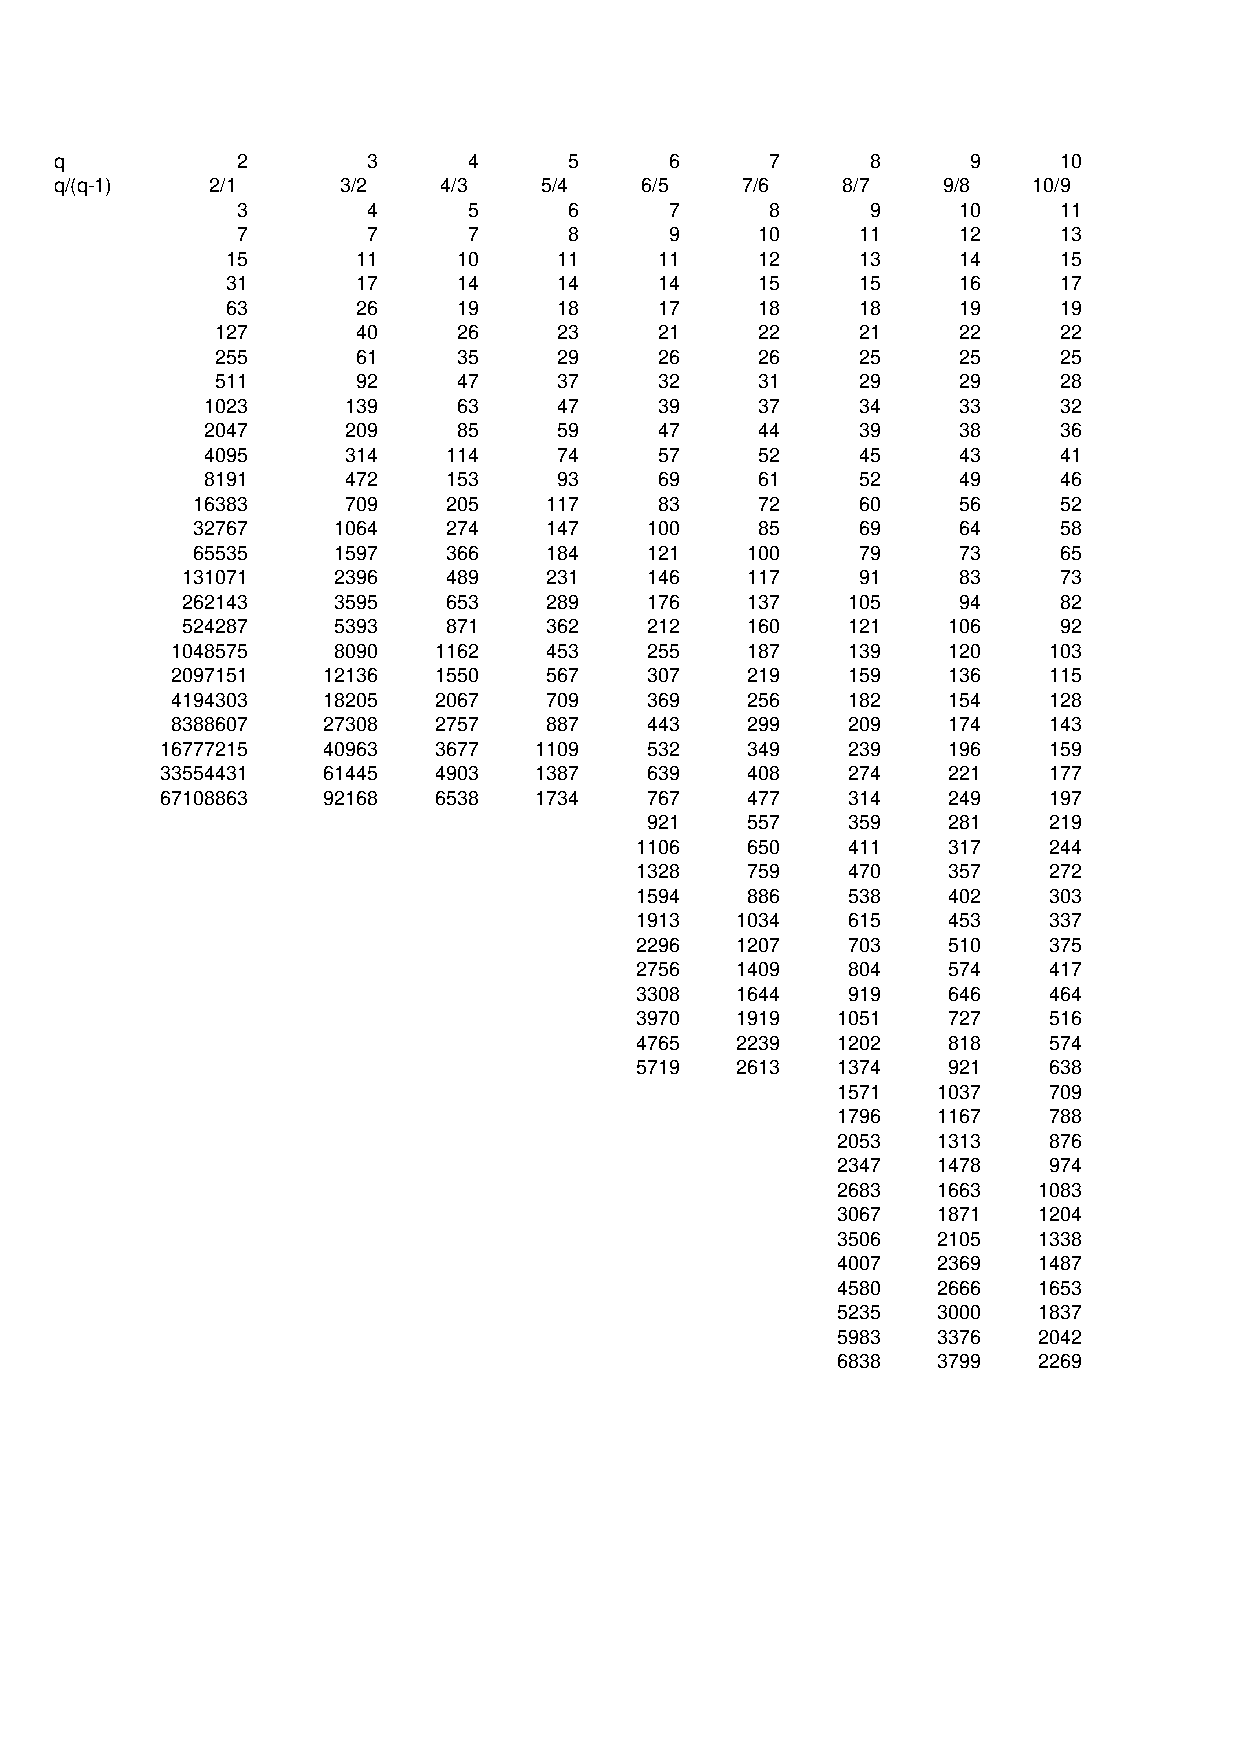
\includegraphics[width=1.0\textwidth]{JosephusTabel}
En sådan tabel er vist her for \(q\) op til \(10\). Hvis for eksempel \(q=5\) og \(n=15\) skal vi finde den største \(d\) således at \(0<nq-d<n\). Vi ser i kolonnen for \(q=5\) og finder at den største \(d\) der er mindre end \(nq=75\) er \(74\). Derfor er overleveren \(75-74=1\).
